%%%%%%%%%%%
% PREÁMBULO
%%%%%%%%%%%

% Todos los paquetes necesarios para muchas funciones especiales del documento están en el documento config.tex. Se colocan en un documento separado para que el principal sea más ordenado.
% Paquetes de generalidades
%%%%%%%%%%%%%%%%%%%%%%%%%%%%%%%

%-----------------------------------------------------------
% defino el formato del documento
\documentclass[a4paper,12pt]{article}
\usepackage[utf8]{inputenc}
\usepackage[spanish]{babel}
\usepackage{csquotes}
\usepackage[a4paper]{geometry}%
\geometry{
  a4paper,
  left       =10mm,
  right      =10mm,
  top        =30mm,
  bottom     =15mm,
  headheight =20mm
}
%-----------------------------------------------------------

% Paquetes para matemática
%%%%%%%%%%%%%%%%%%%%%%%%%%%%%%%

% Los paquetes ams son desarrollados por la American Mathematical Society y mejoran la escritura de fórmulas y símbolos matemáticos.
\usepackage{amsmath}
\usepackage{amsfonts}
\usepackage{amssymb}

% Paquetes para manejo de gráficas y figuras
%%%%%%%%%%%%%%%%%%%%%%%%%%%%%%%


% para tabular graficos tablas y ecuaciones
\usepackage{tabularx}

\usepackage{multirow}


% Para insertar gráficas
\usepackage{graphicx}

% Para colocar varias subfiguras
\usepackage[lofdepth,lotdepth]{subfig}

% Para crear gráficos vectoriales con un lenguaje descriptivo/geométrico
\usepackage{tikz}

% Para crear circuitos vectoriales basados en TikZ
\usepackage[american]{circuitikz}

% Paquetes relacionados con el estilo
%%%%%%%%%%%%%%%%%%%%%%%%%%%%%%%

% Para la presentación correcta de magnitudes y unidades
\usepackage{siunitx}

% Para hipervínculos y marcadores
\usepackage[colorlinks=true,urlcolor=blue,linkcolor=black,citecolor=green]{hyperref}
	\urlstyle{same}

% Para ubicar las tablas y figuras justo después del texto
\usepackage{float}

% Para hacer tablas más estilizadas
\usepackage{booktabs}

% Para hacer secciones con múltiples columnas
\usepackage{multicol}

% Para insertar código fuente estilizado
\usepackage{listings}
	\lstset{basicstyle=\ttfamily,breaklines=true}
    \lstset{numbers=left, numberstyle=\tiny, stepnumber=1, numbersep=6pt}

% Para agregar código con formato de Matlab
\usepackage[numbered,autolinebreaks]{mcode}

% Para utilizar el número de páginas
\usepackage{lastpage}

% Para manejar los encabezados y pies de página
\usepackage{fancyhdr}
	% Contenido de los encabezados y pies de pagina
	\pagestyle{fancy}

%Para cambiar la orientación del texto
\usepackage[document]{ragged2e}

% Misceláneos
%%%%%%%%%%%%%%%%%%%%%%%%%%%%%%%
\usepackage{enumitem}
\usepackage{verbatim}


% Para insertar símbolos extraños
\usepackage{marvosym}

\usepackage{pdfpages}



  \lhead{
\includegraphics[height=1.5cm]{lhead}} %PNG DE FACULTAD
  \chead{
    {\scshape 86.06 - Circuitos Electrónicos} \\
    \vspace{2mm}
    {\large \textbf{TL2: Etapas con Transistores Discretos}}
    \vspace{1mm}
  }
  \rhead{Turno Tarde - \textcolor{blue}{Informe}}
  \lfoot{Facultad de Ingeniería}
  \cfoot{\thepage\ de \pageref{LastPage}}
  \rfoot{Universidad de Buenos Aires}

% Comandos especiales
\newcommand{\EIE}{\textsc{FIUBA \Lightning~ Ingeniería Electrónica}}
\usepackage{ upgreek }
\usepackage[backend=biber]{biblatex} % I try to use biber.

\newcommand{\imgdir}{imgs}
\graphicspath{{\imgdir/}}

%this might not work in online TeX compilers
\addbibresource{ref.bib} % the ref.bib file

% and this should work
%\bibliography{./ref} % the ref.bib file

%%%%%%%%%%%%%%%%
\begin{document}	% Inicio del documento

    \begin{center}
        \textbf{Grupo 6}\\
        \medskip
        González, Jose ....................... jfgonzalez@fi.uba.ar\\
        Urquiza, Elías ........................ eurquiza@fi.uba.ar\\
				Gottfried, Joel .............. joelgottfried99@gmail.com\\
        \medskip
        \emph{2° Cuatrimestre 2019}\\
        18/10/19
    \end{center}
    %%%%%%%%%%%%%%%%%%%%%%
    %Informe
    %%%%%%%%%%%%%%%%%%%%%%
    \begin{multicols}{2}
    \justifying
        \section{Objetivos}

        \section{Resumen}

        \section{Parte A: Etapa amplificadora con un transistor}

        \subsection{Especificaciones}

        Necesitamos diseñar una etapa amplificadora con un transistor \textbf{JFET 2N5486} donde la ganancia de potencia sea $G_p > 100$.

        \subsection{Diseño}

        \begin{center}
                   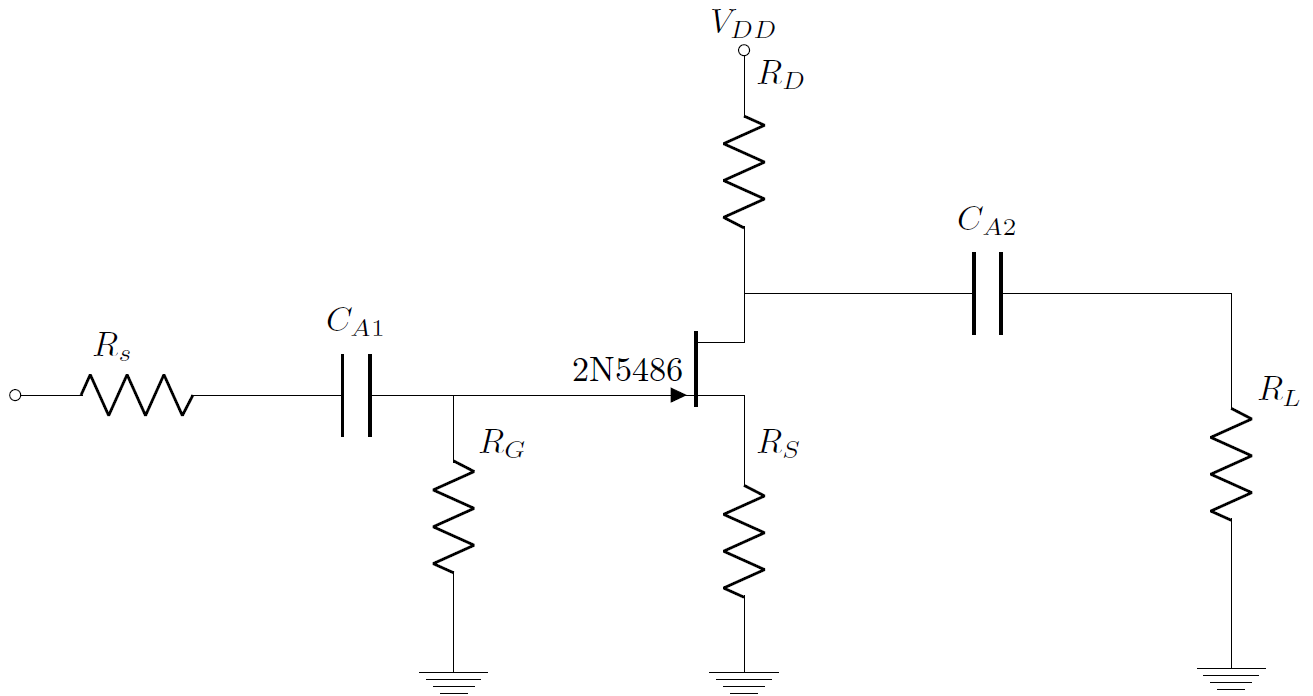
\includegraphics[width=\columnwidth]{diseno1.png}
                   \captionof{figure}{Etapa Amplificadora - Source Común.}
        \end{center}


        El circuito propuesto consiste en un JFET Canal N en modo Source Común con una camino de realimentación. Para este circuito definimos la ganancia de potencia para señales senoidales como

        \begin{equation}
        	G_P = \frac{P_O}{P_I} = \frac{\hat{V_O}\hat{I_O}/2}{\hat{V_S}\hat{I_S}/2} = \frac{\hat{V_O}\hat{I_O}}{\hat{V_S}\hat{I_S}} = A_{vs}\cdot A_{i}
        	\end{equation}

        De la hoja de datos se obtienen los datos para definir una \textbf{zona de operación segura} de la Figura \ref{fig:zona_segura} dentro de los cuales podremos polarizar al transistor.



        \begin{center}
                   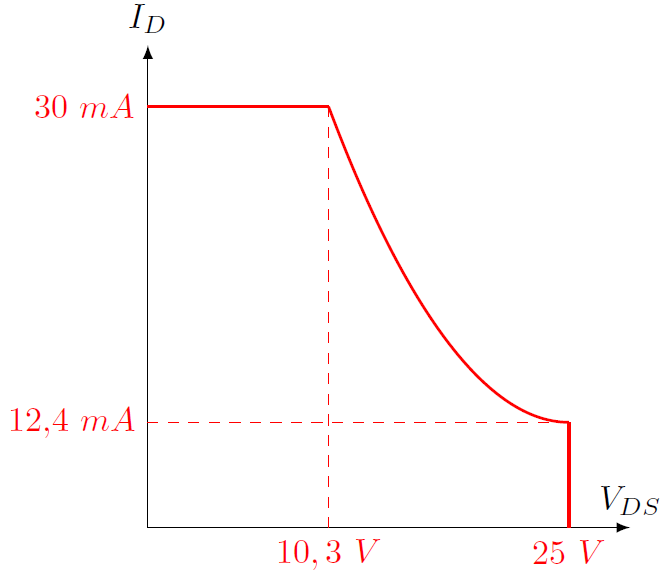
\includegraphics[width=\columnwidth]{diseno2a.png}
                   \captionof{figure}{Zona de operación segura del transistor.}
                   \label{fig:zona_segura}
        \end{center}

        \begin{center}
                   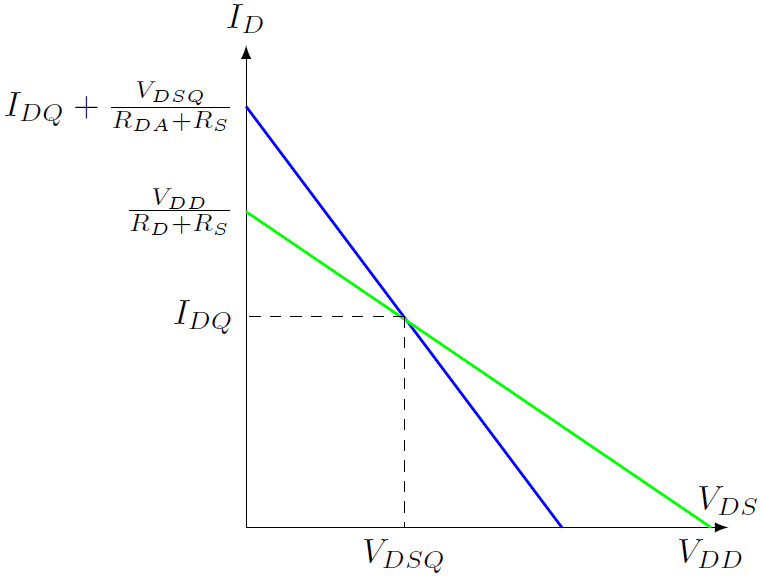
\includegraphics[width=\columnwidth]{diseno2b.png}
                   \captionof{figure}{Rectas de carga para el circuito propuesto.}
                   \label{fig:rectas_carga}
        \end{center}



        \subsubsection{Rectas de Carga}


        \begin{center}
                   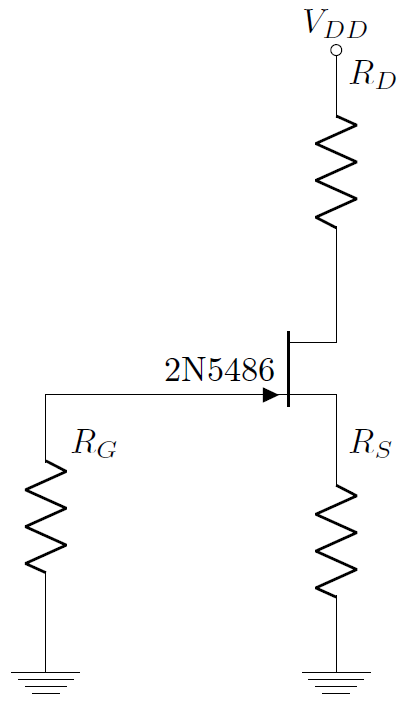
\includegraphics[width=.3\columnwidth]{diseno3.png}
                   \captionof{figure}{Etapa Amplificadora - Circuito de Continua.}
                   \label{fig:circuito_continua}
        \end{center}

        En la Figura \ref{fig:circuito_continua} se ve el circuito de continua, donde la recta de carga estática se obtiene al recorrer la malla de salida:

        \begin{equation}
        	I_D = \frac{V_{DD}}{R_D + R_S} - \frac{V_{DSQ}}{R_D + R_S}
        	\end{equation}

        y la recta de carga dinámica será

        \begin{equation}
        	i_D = \frac{-1}{(R_D//R_L) + R_S}\cdot v_{DS} + I_{DQ} + \frac{V_{DSQ}}{(R_D//R_L) + R_S}
        	\end{equation}


        \subsubsection{Parámetros de pequeña señal}



        \begin{center}
                   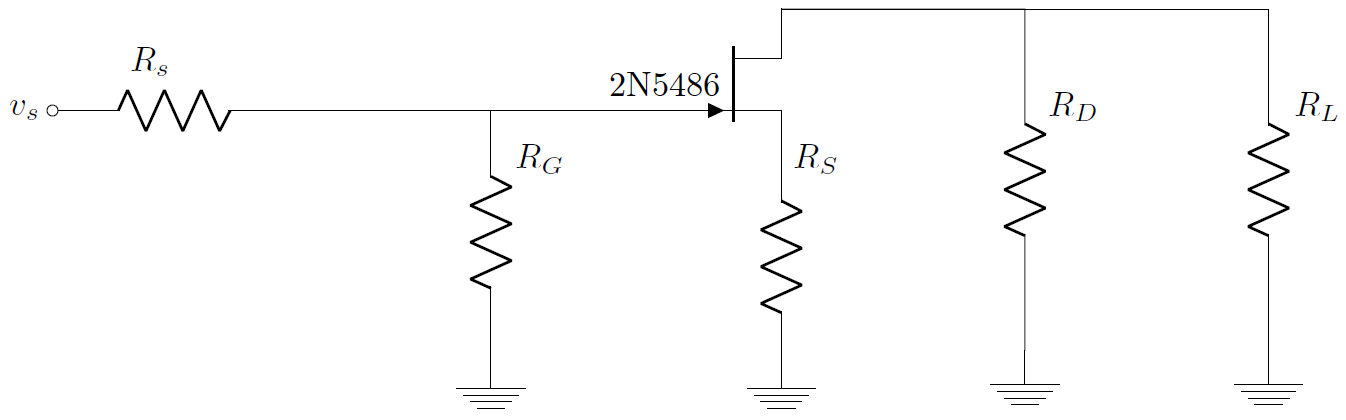
\includegraphics[width=\columnwidth]{diseno4.png}
                   \captionof{figure}{Etapa Amplificadora - Circuito de señal a frecuencias medias.}
                   \label{fig:circuito_señal}
        \end{center}



        Del circuito de señal a frecuencias medias podemos obtener los siguientes parámetros por inspección, en una primera aproximación \textbf{despreciando efectos de segundo orden en el transistor}.
        La ganancia de tensión será

        \begin{equation}
        A_v = \frac{v_o}{v_i} = \frac{-i_o(R_D // R_L)}{v_{gs}+ v_{R_S}} = \frac{-(R_D//R_L)}{\frac{v_{gs}}{i_o}+R_S} = \frac{-(R_D//R_L)}{\frac{1}{g_m}+R_S}
        \end{equation}

        que referida al generador resulta

        \begin{equation}
        A_{vs} = A_v \frac{v_i}{v_s} = A_v \frac{R_G}{R_G + R_s}
        \end{equation}

        La ganancia de corrientes será

        \begin{equation}
        A_i = \frac{i_o}{i_s} = \frac{i_o}{\frac{v_i}{R_G}} = \frac{i_o}{v_{gs}+i_o R_S} = \frac{R_G}{\frac{1}{g_m}+R_S}
        \end{equation}

        Asumiendo que se cumple que $R_S >> 1/g_m$ y $R_s << R_G$ \textbf{se puede expresar la ganancia de potencia en una primera aproximación que depende integramente de la elección de resistencias}

        \begin{equation}
        G_P = A_{vs}\times A_i \approx \frac{R_D//R_L}{R_S} \times \frac{R_G}{R_S}
        \end{equation}


        la resistencia de entrada y salida serán:

        \begin{equation}
        R_I = R_G
        \end{equation}

        \begin{equation}
        R_O = R_D(1+g_mR_S)
        \end{equation}


        \subsubsection{Elección de valores}

        Con el objetivo de obtener $G_P > 100$ se eligieron los valores de resistencias y fuente de polarización del Cuadro \ref{tab:valores}.

        \begin{table}[h]
        \centering
        \begin{tabularx}{0.7\textwidth}{XXXXX}
        \hline
         $R_G$  		& $R_D$ 		& $R_S$ 			& $R_L$ 		& $V_{DD}$ \\
         \hline
         $820\ k\Omega$ & $1\ k\Omega$ 	& $470\ k\Omega$ 	& $10\ k\Omega$ & $12\ V$ \\
        \hline
        \end{tabularx}
        \caption{Valores propuestos para la etapa amplificadora.}
        \label{tab:valores}
        \end{table}



        \subsubsection{Dispersión de parámetros}

        En el Cuadro \ref{tab:dispersion} se muestran los distintos parámetros del amplificador y el punto de reposo para los valores extremos de los parámetros $I_{DSS}$ y $V_P$ del JFET con la elección de resistencias de la sección anterior.



        \begin{table}[h]
        \centering
        \begin{tabularx}{1\textwidth}{XXXXXXXX}
        \hline
        \multicolumn{2}{c}{}				& \multicolumn{4}{c}{Parámetros del Amplificador}						& \multicolumn{2}{c}{Punto de Reposo} \\
        									\cmidrule(r){3-6}														\cmidrule(r){7-8}
        \multicolumn{2}{c}{$(I_{DSS},V_{P})$}& $|A_{vs}|$  		& $|A_{i}|$ 		& $G_P$ 			& $g_m$ 		& $I_{DQ}$ 			& $V_{DSQ}$			\\
        \cmidrule(r){1-2}  									\cmidrule(r){3-3} \cmidrule(r){4-4} 	\cmidrule(r){5-5} 	\cmidrule(r){6-6} \cmidrule(r){7-7} 	\cmidrule(r){8-8}
        \multicolumn{2}{c}{$(20\ mA,-6\ V)$}& $1.2$	& $1096$	& $1316$ & $3.6\ mA/V$ & $5.8\ mA$& $3.5\ V$\\
        \hline
        \multicolumn{2}{c}{$(14\ mA,-4\ V)$}& $1.2$	& $1108$	& $1329$ & $3.7\ mA/V$& $3.9\ mA$ & $6.3\ V$\\
        \hline
        \multicolumn{2}{c}{$$(8\ mA,-2\ V)$$}&$1.3$	& $1139$	& $1480$ & 4\ mA/V & $2\ mA$ & $9.1\ V$ \\
        \hline
        \hline
        \multicolumn{2}{c}{\textcolor{red}{Dispersión:}} & $8\%$ & $3\%$ & $13\%$ & $11\%$ & $190\%$ & $160\% $\\
        \hline
        \end{tabularx}
        \caption{Parámetros teóricos de la etapa amplificadora.}
        \label{tab:dispersion}
        \end{table}

        Para obtener estos valores se tuvieron en cuenta los siguientes puntos

        \begin{itemize}
        	\item En ningún caso se cumple $1/g_m << R_S$ luego se usaron las expresiones completas de ganancias.
        	\item Se despreciaron efectos de segundo orden en el transistor.
        	\item Se utilizó para describir la dispersión el rango porcentual respecto al mínimo dado por
        		\begin{equation}
        		\delta f \% = \frac{f_{MAX}-f_{MIN}}{f_{MIN}}\times 100 \nonumber
        		\end{equation}
        	\item Se asumieron valores típicos como los valores promedios a falta de esta información en hoja de datos.

        	\end{itemize}


        En la Figura \ref{fig:dispersion} se muestran los distintos puntos de reposo en el contorno de la zona segura.

        \begin{center}
                   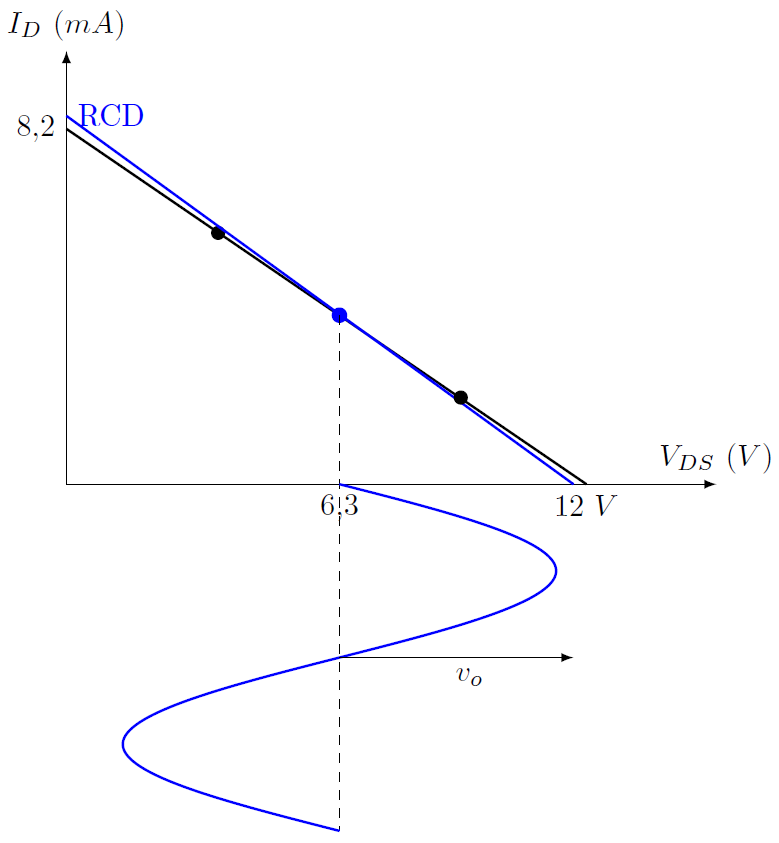
\includegraphics[width=\columnwidth]{diseno5.png}
                   \captionof{figure}{Recta de carga estática con puntos de reposo extremos y típico.}
                   \label{fig:dispersion}
        \end{center}


        \subsubsection{Realimentación en señal}

        El circuito presenta un camino de realimentación de señal de muestreo de corriente y suma de tensión. En la Figura \ref{fig:realimentacion} se hace un análisis de incrementos para mostrar que la realimentación es negativa.


        \begin{center}
                   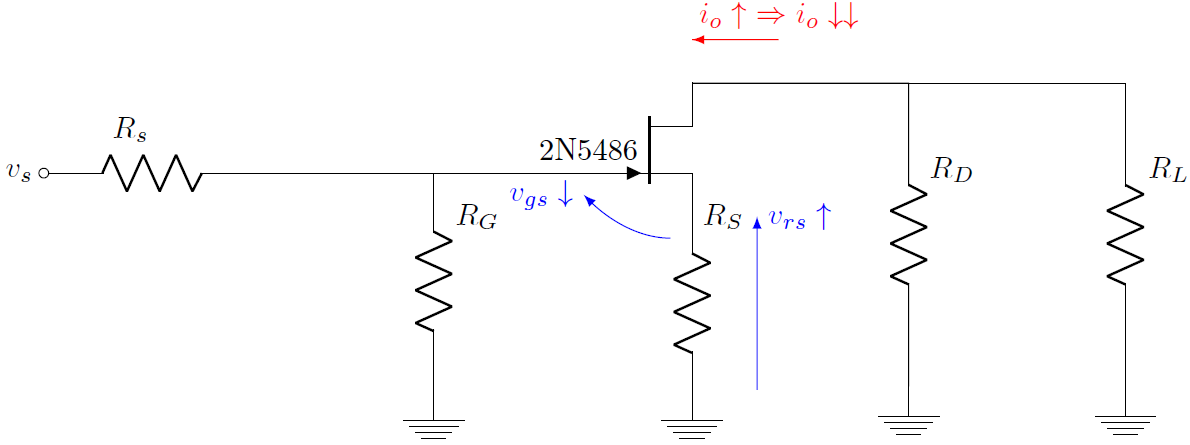
\includegraphics[width=\columnwidth]{diseno6.png}
                   \captionof{figure}{Análisis de incrementos de la realimentación.}
                   \label{fig:realimentacion}
        \end{center}


        De las expresiones de ganancia de tensión podemos obtener que el \textbf{factor de realimentación} para este circuito es
        \begin{equation}
        	FR = 1+g_mR_S
        	\end{equation}

        \subsubsection{Señales sin recorte}

        Asumiendo el punto de operación Q asociado a los valores típicos del transistor $I_{DSS} = 14\ mA$ y $V_P = -4\ V$ obtenemos las máximas señales sin distorsión. De la Figura \ref{fig:dispersion} se ve que para los valores típicos la máxima tensión a la salida sin distorsión por recorte ni triodo serán de tensión máxima aproximadamente $\hat{v_o} = 6\ V$. Luego, en este punto la ganancia referida al generador es de unos $A_{vs} = 1.2$, entonces la máxima tensión que podemos poner del generador, a valores típicos, será

        \begin{equation}
        	v_s = \frac{v_o}{A_{vs}} \approx 5\ V \nonumber
        	\end{equation}

        \textbf{El límite por alinealidad será el determinante de las máximas señales del generador}. Aceptando un error del $10\ \%$ en la linealización se obtiene una cota de $v_{gs} < 25\ mV$ asociado a la tensión térmica.

        \begin{equation}
        	v_{gs} = 25\ mV \Rightarrow v_o = -i_o\times R_D//R_L = -g_m\cdot v_{gs} \times R_D//R_L = - 80\ mV \Rightarrow v_s = 67\ mV
        	\end{equation}

        \textbf{La máxima amplitud pico de señal que puede tener el generador sin distorsión de ningún tipo es $v_s = 67\ mV$ (cuando $I_{DSS} = 14\ mV$ y $V_P = -4\ V$).}

        \newpage

        \section{Parte D: Oscilador Senoidal por desplazamiento de fase}

        \begin{center}
                   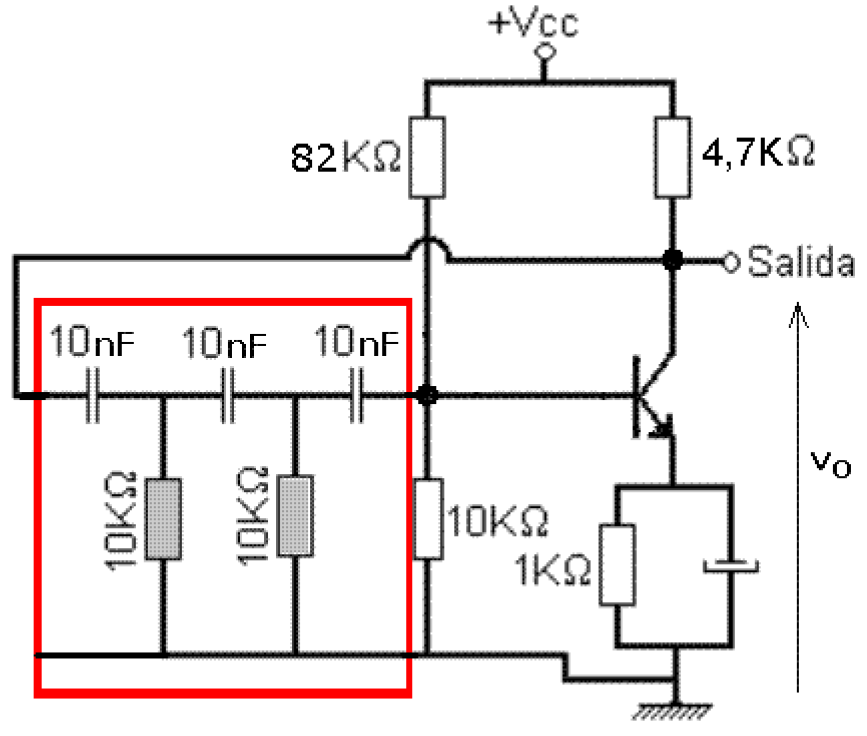
\includegraphics[width=\columnwidth]{oscilador1.png}
                   \captionof{figure}{Oscilador Senoidal "Phase-Shift" con $V_{CC}=20V$.}
                   \label{fig:oscilador}
        \end{center}

        \subsection{Explicación Cualitativa}

        \subsection{Análisis de Realimentación}

        \subsection{Simulación}

        \begin{center}
                   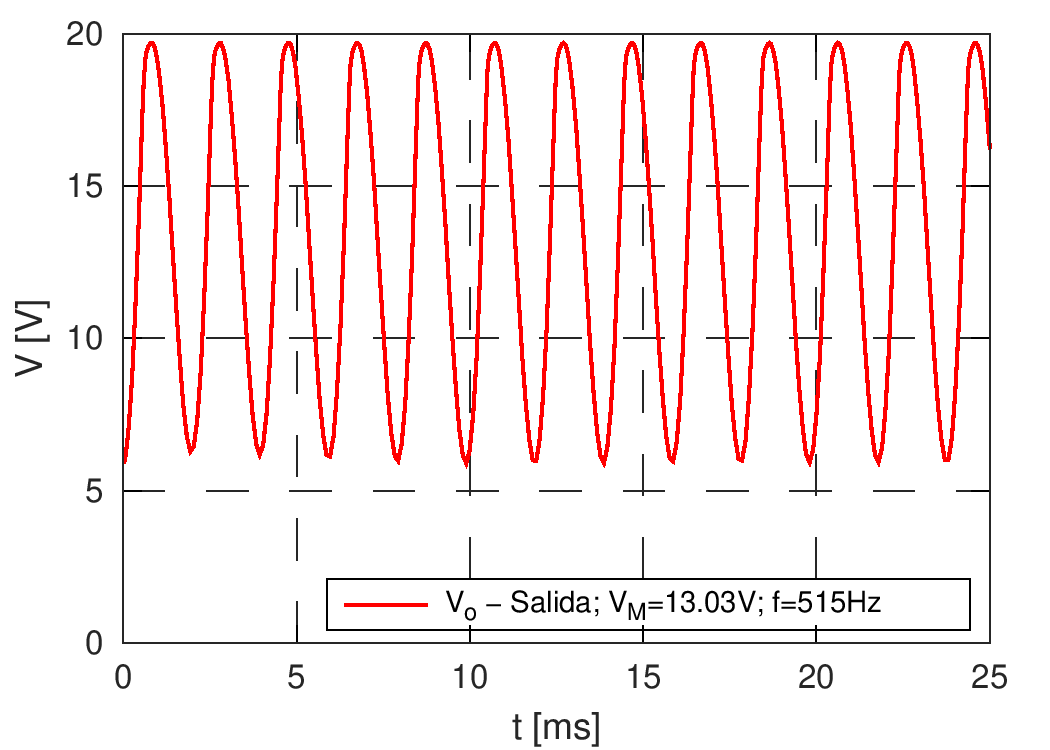
\includegraphics[width=\columnwidth]{salida_oscilador.png}
                   \captionof{figure}{Señal de salida del oscilador.}
                   \label{fig:sim_out_oscilador}
        \end{center}

        \begin{center}
                   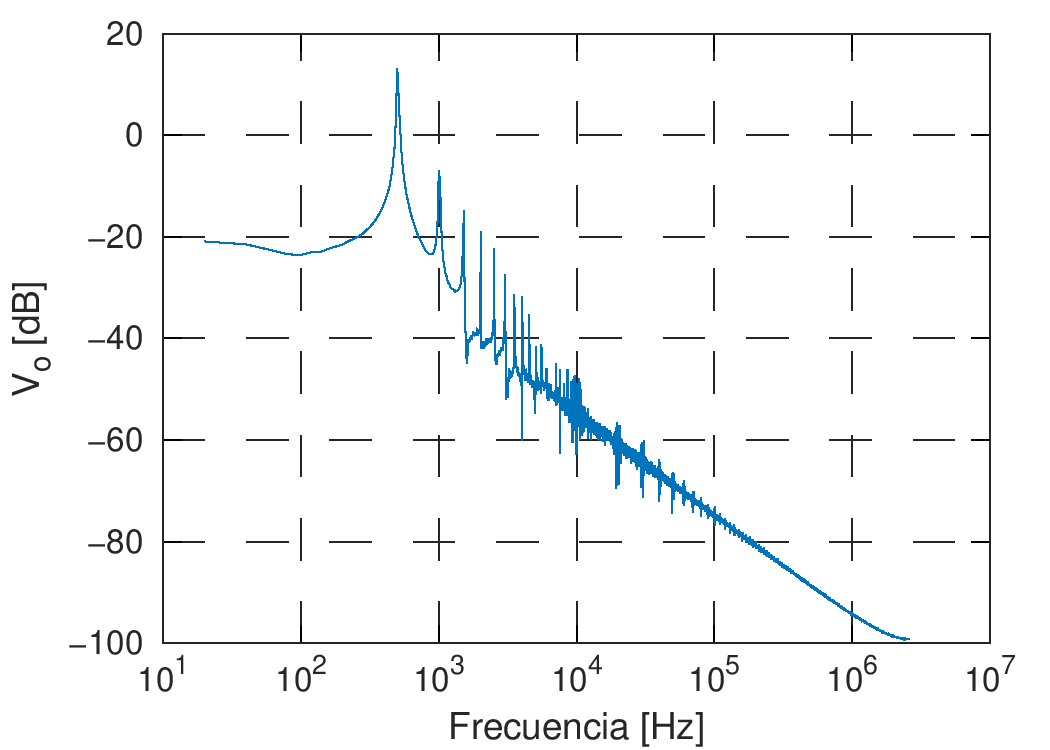
\includegraphics[width=\columnwidth]{fft_oscilador.png}
                   \captionof{figure}{FFT de la señal de salida del oscilador.}
                   \label{fig:fft}
        \end{center}

        \section{Conclusiones}

        \section{Referencias} %Usar \printbibliography y el archivo ref.bib
        \begin{itemize}
            \item How Oscilloscope Probes Affect Your Measurement - Application Note - Tektronix
        \end{itemize}
        %\printbibliography

    \end{multicols}
\end{document}
